\begin{appendices}

%\chapter{Initial Project Plan}
%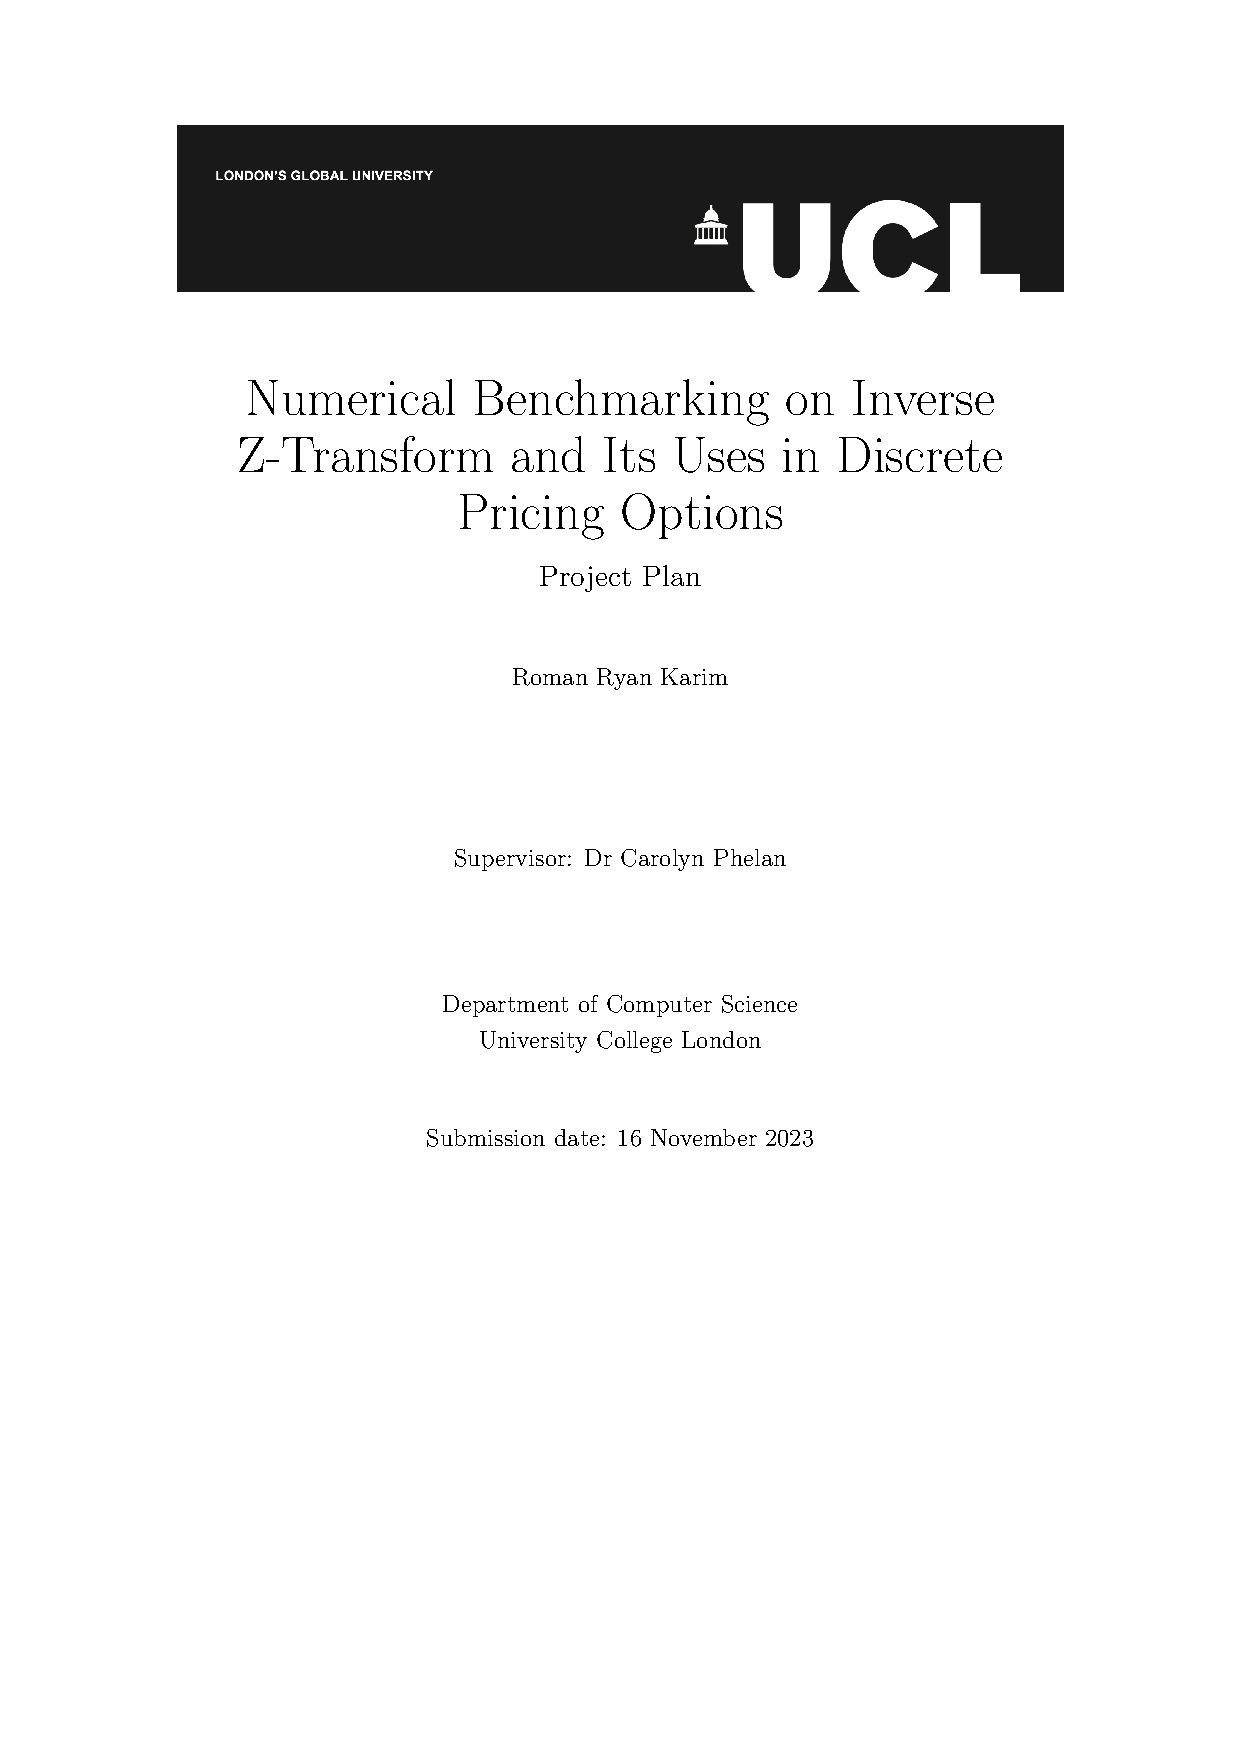
\includepdf[pages=-]{initial_project_plan.pdf}

\chapter{Code Listings}\label{chapter:code_listings}

% ========================================
% Transform Pairs
% ========================================
\section{Transform Pairs}
These transform pairs serve as benchmarks for testing the accuracy and efficiency of numerical inversion methods. Each pair consists of a time-domain function and its corresponding Z-transform, providing a practical basis for analysing and validating the implemented algorithms. The code is given in Python.

\subsection{Heaviside Step}
\begin{lstlisting}[language=Python, caption= Implementation of the Heaviside Step function and its $\mathcal{Z}$-transform (Section \ref{section:heaviside_step})]
def f(t):
    return 1
    
def ftilde(z):
    return z / (z-1)
\end{lstlisting}

\subsection{Polynomial}
\begin{lstlisting}[language=Python, caption= Implementation of the Polynomial function and its $\mathcal{Z}$-transform (Section \ref{section:polynomial})]
def f(t):
    return t
    
def ftilde(z):
    return z / (z-1)**2
\end{lstlisting}

\subsection{Decaying Exponential}
\begin{lstlisting}[language=Python, caption= Implementation of the Decaying Exp function and its $\mathcal{Z}$-transform (Section \ref{section:decaying_exp})]
def f(a, t):
    return np.exp(-a * t)
    
def ftilde(z, a, t, N):
    delta_t = t / N
    denominator = 1 - np.exp(-a * delta_t) / z
    return 1 / denominator
\end{lstlisting}

\newpage
\subsection{Sinusiodal}
\begin{lstlisting}[language=Python, caption= Implementation of the Sinusoidal function and its $\mathcal{Z}$-transform (Section \ref{section:sinusoidal})]
def f(omega, t):
    return np.sin(omega * t)
    
def ftilde(z, omega, t, N):
    delta_t = t / N
    numerator = z**(-1) * np.sin(omega * delta_t)
    denominator = 1 - 2 * np.cos(omega * delta_t) * z**(-1) + z**(-2)
    return numerator / denominator
\end{lstlisting}

\newpage
\section{Contours}

\subsection{Circular}
\begin{lstlisting}[language=Python, caption= null]
def circle(r, n):
    z = []
    for k in range(0, n):
        theta = np.pi * k / n
        point = r * np.exp(1j * theta)
        z.append(point)
    return z
\end{lstlisting}

\begin{lstlisting}[language=Python, caption= null]
def circle(r, n):
    z = []
    for k in range(0, n):
        theta = (np.pi + np.pi / n) * k / n
        point = r * np.exp(1j * theta)
        z.append(point)
    return z
\end{lstlisting}

\subsection{Sinh Deformation}
\begin{lstlisting}[language=Python, caption= null]
def hyperbolic_sine(sigma, b, y, n):
    z = np.zeros(n, dtype=complex)
    for k in range(-n//2, n//2):
        omega = 1j * (np.pi) * k / n
        z[k + n//2] = sigma + 1j * b * np.sinh(omega + y)
    return z
\end{lstlisting}

\begin{lstlisting}[language=Python, caption= null]
def hyperbolic_sine(sigma, b, y, n):
    z = np.zeros(n, dtype=complex)
    for k in range(-n//2, n//2):
        omega = 1j * (np.pi + np.pi / n) * k / n
        z[k + n//2] = sigma + 1j * b * np.sinh(omega + y)
    return z
\end{lstlisting}

% ========================================
% Numerical Inverse Z-Transform
% ========================================
\newpage
\section{Numerical Inverse $\mathcal{Z}$-Transform}

\subsection{Abate and Whitt 1992}
\begin{lstlisting}[language=Python, caption= null ]
def abate_whitt(ftilde, n, lmbda):
    rho = 10 ** (-lmbda / (2 * n))

    summation = 0
    for k in range(1, n):
        z = 1 / (rho * np.exp(1j * k * np.pi / n))
        term = ftilde(z)
        summation += ((-1)**k) * np.real(term)
    summation *= 2
    
    start = ftilde(1 / rho)
    end = ((-1)**n) * ftilde(1 / -rho)
    scale_factor = 1 / (2 * n * rho**n)

    result = scale_factor * (start + summation + end)

    return result
\end{lstlisting}

\subsection{Cavers 1978}
\begin{lstlisting}[language=Python, caption= null]
def cavers(ftilde, n, N, gamma):
    r = 10 ** (gamma / (N))
    k = np.arange(N)
    z = r * np.exp(1j * 2 * np.pi * k / (N))
    F = np.fft.ifft(ftilde(z))
    f = r ** n * F[n]
    return f
\end{lstlisting}

\begin{lstlisting}[language=Python, caption= null]
def cavers_dft(ftilde, n, J, gamma):
    N = n[-1]
    r = 10 ** (gamma / J)
    
    j = np.arange(J) # secondary grid points
    z = r * np.exp(1j * 2 * np.pi * j / J)
    
    f = np.zeros(N + 1, dtype=complex)
    for i in range(N + 1):
        f[i] = np.sum(z**n[i] * ftilde(z)) / J
    return f
\end{lstlisting}

% ========================================
% Optimisation Techniques
% ========================================
\newpage
\section{Optimisation Techniques}

\subsection{Loss Function}
\begin{lstlisting}[language=Python, caption= null]
def loss(z):
    L1 = np.sum((np.abs(z) - 1) ** 2)
    return L1
\end{lstlisting}

\subsection{Gradient Descent}
\begin{lstlisting}[language=Python, caption= null]
def gradient_descent(N, learning_rate=1e-3, num_iterations=1_000_000):
	# initial values
    b = 0.7
    y = 0.895588
    
    # initialising parameters
    best_loss = float('inf')
    best_b = b
    best_y = y

    for i in range(num_iterations):
        # compute loss
        L1 = loss_function(b, y, N)
        
        if L1 < best_loss:
            best_loss = L1
            best_b = b
            best_y = y
        
        # compute gradients 
        epsilon = 1e-8
        grad_b = (loss_function(b + epsilon, y, N) - L1) / epsilon
        grad_y = (loss_function(b, y + epsilon, N) - L1) / epsilon
        
        # update parameters
        b -= learning_rate * grad_b
        y -= learning_rate * grad_y
    
    return best_b, best_y, best_loss
\end{lstlisting}

\subsection{ADAM Optimiser}
\begin{lstlisting}[language=Python, caption= null]
def adam_optimiser(N, initial_learning_rate=1e-3, num_iterations=1_000_000, beta1=0.9, beta2=0.999, epsilon=1e-5):
	# initial values
    b = 0.14124692711511863
    y = 2.6503746377415633

	# initialising parameters
    best_loss = float('inf')
    best_b = b
    best_y = y
    m_b, v_b = 0, 0
    m_y, v_y = 0, 0
    t = 0

    for i in range(num_iterations):
        t += 1
        
        # compute loss
        L1 = loss_function(b, y, N)
        
        if L1 < best_loss:
            best_loss = L1
            best_b = b
            best_y = y
        
        # compute gradients (estimate)
        grad_b = (loss_function(b + epsilon, y, N) - L1) / epsilon
        grad_y = (loss_function(b, y + epsilon, N) - L1) / epsilon
        
        # update biased first moment
        m_b = beta1 * m_b + (1 - beta1) * grad_b
        m_y = beta1 * m_y + (1 - beta1) * grad_y
        
        # update biased second moment
        v_b = beta2 * v_b + (1 - beta2) * (grad_b ** 2)
        v_y = beta2 * v_y + (1 - beta2) * (grad_y ** 2)
        
        # compute bias-corrected first moment
        m_b_hat = m_b / (1 - beta1 ** t)
        m_y_hat = m_y / (1 - beta1 ** t)
        
        # compute bias-corrected second moment
        v_b_hat = v_b / (1 - beta2 ** t)
        v_y_hat = v_y / (1 - beta2 ** t)
        
        # update parameters
        b -= initial_learning_rate * m_b_hat / (np.sqrt(v_b_hat) + epsilon)
        y -= initial_learning_rate * m_y_hat / (np.sqrt(v_y_hat) + epsilon)
       
    return best_b, best_y, best_loss
\end{lstlisting}

  
\end{appendices}